\section {Introduction to the analysis}

In this note, we present initial results of the tracker DAQ commissioning.
\section{Description of teststand setup}
The tracker test stand,  TS1, included one DRAC card connected via an optical fiber
to the DTC installed in the DAQ computer mu2edaq09, 96 channels in total.
The ROC was operated in two different data readout modes:
\begin{itemize}
\item 
  mode 1: the ROC was emulating the data itself without reading FPGAs (a pattern readout mode).
\item 
  mode 2: the ROC was reading digi FPGAs.
\end{itemize}

Most of the data were taken operating in the mode 2, with digi FPGAs, pulsed by their internal pulsers.
A pulser has two different frequencies,  31.29 MHz/(2$^7$+1), or approximately 250 kHz, 
and 31.29 MHz/(2$^9$+1), or approximately 60 kHz.
Event window is the time interval between two heartbeats (HB's). 
A timing diagram of a single channel readout is shown in Fig. \ref{fig:3}.
Pulses, separated by $T_{gen}=1/f_{gen}$, where $f_{gen}$ is the generator frequency
are represented by gray triangles.
The event window, with the width of $T_{EW}$, that represents the distance between the proton pulses, 
was varied from 700 ns to 50 $\mu$s. 
The ROC firmware has an internal hit buffer which stores up to 255 hits.
Depending on $T_{gen}$ and $T_{EW}$, the data taking can proceed in two different
scenarios:
\begin{itemize}
\item
  The event window is large enough , so the total number of generated hits is greater than 255. In this case
  the ROC hit buffer always gets filled up, and only the first 255 hits are read out;
\item
  The total number of hits within the event window is less than 255.
  In this case the ROC hit buffer doesn't get filled up and the total number of hits may vary from one event to another.
\end{itemize}

Each digi FPGA has its own pulse generator and the pulse sequences from the two
generators are offset with respect to each other by a time interval $\Delta t$.
The offset is constant for as long as the DRAC board is powered up and varies randomly between 0 and $T_{gen}$ when DRAC is powercycled.
The timing of the readout is uncorrelated with the generator timing sequences,
  so the number of pulses within the readout window can vary from  from one event to another, as shown
  in Figure \ref{fig:3}.

Relative timing offsets of the channels within the same FPGA are of the order of a few nanoseconds.
The channel readout sequence is fixed and is presented in Appendix \ref{order}.

\begin{figure}[!h]
\centering
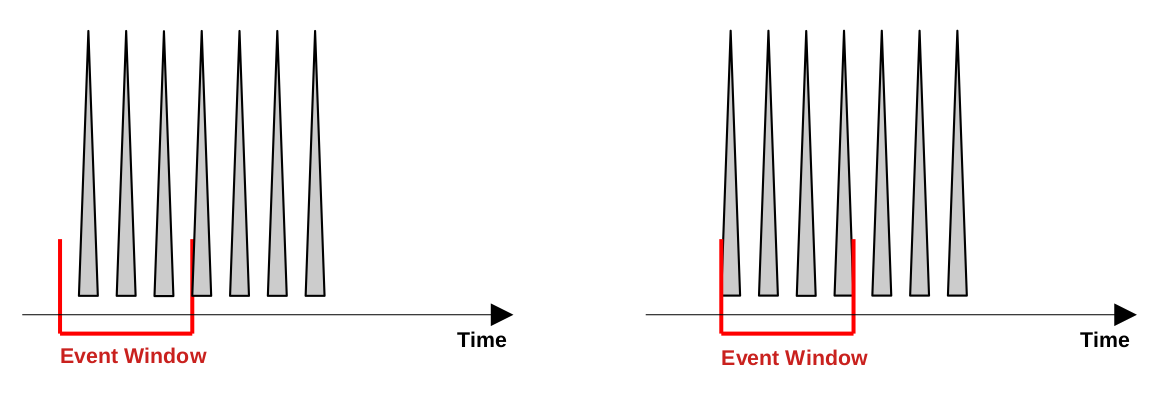
\includegraphics[width =0.8\textwidth]{figures/pdf/finalimg}
\caption{Graphic illustration of pulses in an event window.}
\label{fig:3}
\end{figure}

The data taking has been performed using OTSDAQ+ARTDAQ software, and for each run the output data
have been stored in an art file moved to {\bf /exp/mu2e/data/projects/tracker/vst} area mounted
on Mu2e central platforms.


%%%%%%%%%%%%%%%%%%%%%%%%%%%%%%%%%%%%%%%%%%%%%%%%%%%%%%%%%%%%%%%%%%%%%%%%%%%%%%
\section{Monte Carlo simulation}\label{MonteCarlo}
 
The ROC readout logic is purely digital, so the readout process can be simulated. 
The logic of the simulation is as follows.
The simulated parameters for each event are the number of hits in each channel
and the total number of readout hits.

In the following sections, we call $occupancy$ the total number of hits
recorded in a given channel during the test run.

Given that the total number of hits per event doesn't exceed 255, the simulation follows these steps:
\begin{itemize}
\item
  The event window starts at $t=0$s;
\item
  In a given FPGA, the timing of the first pulse is generated randomly from 0 to $T_{gen}$
  by sampling a uniform distribution;
\item
  The subsequent pulses are added, separated from each other by $T_{gen}$,
  until the absolute time
  of the next pulse is greater than $T_{EW}$;
\item
  In the readout part of the simulation, the pulses are read out following the readout sequence;
\item
  the readout ``continues'' until all simulated hits are included or
  the total number of read out hits reaches the maximum threshold of 255. 
\end{itemize}

The simulation also takes into account the offset between the two FPGA timing sequences
and the individual channel-to-channel timing offsets. 
In the following sections, results of the data taking are compared with the simulation.
%%% Local Variables:
%%% mode: latex
%%% TeX-master: t
%%% End:

